\documentclass[../main.tex]{subfiles}

\begin{document}

\section{Human-Machine Ensemble Method}
\label{sec: Human-Machine Ensemble Method}

In this chapter, Section~\ref{sub: Overview} describes the characteristics of forecasts by humans and a machine, and overview the proposed \emph{human-machine ensemble method}.
Then, I modeling the forecasts of humans and ones of machines in Section~\ref{sub: Model}.
Finally, Section~\ref{sub: Optimal Composition of Humans and a Machine} formulates the human-machine ensemble method as a problem to minimize the expected squared error of the ensemble, and solves it.

\subsection{Overview}
\label{sub: Overview}

Traditional ensemble methods assumes that the error of each forecaster always follows a fixed probability distribution as mentioned in Section~\ref{sub: Ensemble Methods}.
However, in fact, since each forecaster has good and weak points, the expected error of each changes depending on the situation.
Let us consider economic forecasts.  Since machines learn past patterns, they are good at a forecasting when the target index follows a pattern, but they are bad when given a pattern not in the past.
On the other hand, humans can consider information such as economy and policies that machines can not lean well, so they are adaptable to patterns not in the past.
Therefore, it is necessary to understand the characteristics of humans and machines for developing a human-machine ensemble method.

\begin{figure}
  \centering
  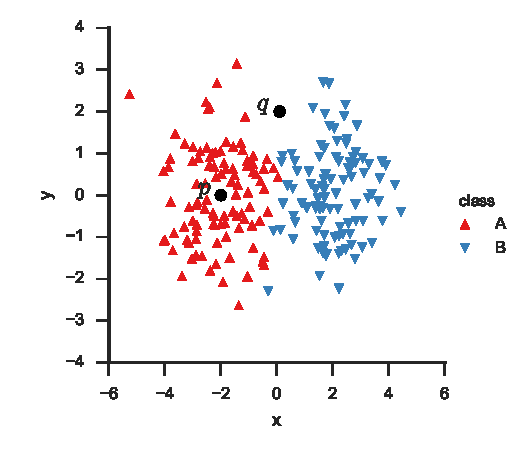
\includegraphics[width=0.6\textwidth]{proposal-machine_example.pdf}
  \caption{
    An illustrative example of a classification problem.
    There are 200 samples represented as points in a 2D feature space.
    Each of them belongs to a class $A$ or $B$.
    Given a sample $p$ as input to a prediction model that learned those samples as training set, the model outputs that the probability of belonging to $A$ is high, while given a sample $q$, the probabilities of belonging to $A$ and $B$ are about the same.
  }\label{fig: example}
\end{figure}

The characteristic of forecasts by machines is that their expected error can be quantified since they make forecasts statistically based on patterns they leaned.
Let us explain by using an illustrative example.
Figure~\ref{fig: example} shows 200 data points belonging to one of two classes $A$ and $B$.
The classes $A$ and $B$ are sampled from the Gaussians with standard deviation $\sigma = 1$ centered at $(-2,0)$ and $(2,0)$, respectively.
Assume that there is a prediction model that learned those samples.
For instance, if this model is given an input $p = (-2,0)$, which has the typical feature of class $A$, it returns that the probability of belonging to $A$ is $0.95$.
Furthermore, given $q=(0.1,2)$, which is located near the boundary of the two classes, it returns the probability is $0.45$.
Of course, humans also can answer the probability that $p$ and $q$ belong to class $A$ based on the figure, but since they answer the probability intuitively, the grounds for the value is weak and the reliability is poor.
Meanwhile, machines can return values with grounds based on the concrete model.

On the other hand, the characteristic of forecasts by humans is that they can make forecasts considering information such as the current economy and new policies, which is difficult for machines to learn.
In addition, forecasts by a group of humans can harness the \emph{wisdom of the crowd} as mentioned in Section~\ref{sub: Wisdom of the Crowd}.
In economic forecasts, opinions are often different among experts, so it is easy to gather diverse forecasts by increasing the number of people.
Conversely, it is difficult to construct diverse prediction models by machine learning.
Even if the learning algorithm is different, the predicted values will be similar since the training set is the same.
Algorithms such as \emph{Random Forest} divide the training set and construct multiple weak learners, but they sacrifices the accuracy of each model.

The human-machine ensemble method combines forecasts of a machine and group of humans according to the expected error of the machine forecast.
In other words, if the expected error of machine is small, the ensemble judge that the machine forecast alone is enough, otherwise it combines forecasts of humans.
This procedure makes it possible to harness the characteristics of machines that can quantify the expected errors and the characteristics of humans that can compensate for the poor part of machines and increase diversity easily.

\subsection{Model}
\label{sub: Model}

In this section, I modeling forecasts of prediction models obtained by machine learning and forecasts of individual humans.
They forecasts continuous values such as annual inflation rate.

\subsubsection{Humans model}
\label{ssub: Humans model}

Forecasts of individual humans are modeled as random variables like Lamberson and Page~\cite{Lamberson2012} introduced in Section~\ref{sub: Ensemble Methods}.
Let random variables $h_i$ and $\varepsilon_{h_i}$ denote the forecast and error of a human $i$.

Assume that the error $\varepsilon_{h_i}$ follows a distribution with mean $\mu = 0$ and variance $\sigma^2 = \varh$.
This means that forecasts by humans are unbiased.
That is, although a forecast can be smaller or greater than the actual value, the positive errors and the negative errors are the same amount as a whole, and the errors are not positively biased or negatively biased.

Moreover, let $H(n)$ denote the average of forecasts by $n$ humans, and let $\covh$ denote the average covariance in the errors of two different humans as
\begin{equation}
  \covh = \frac{1}{n(n - 1)}\sum_{i=1}^n\sum_{j \neq i}\cov(\varepsilon_{h_i}, \varepsilon_{h_j}).
  \label{eq: covh}
\end{equation}
According to~\cite{Ueda1996}, the expected squared error of $H(n)$ is
\begin{equation}
  \MSE(H(n)) = \frac{1}{n}\varh + (1 - \frac{1}{n})\covh.
  \label{eq: expected squared error of humans}
\end{equation}

\subsubsection{Machine model}
\label{ssub: Machine model}

Forecasts of machines are modeled as that the expected error varies according to the input.
The inputs are, for example, inflation fluctuations over the past 12 months.
Assume that a prediction model $\theta$ obtained by machine learning outputs a probability distribution to an input vector $\x$.
This is regarded as the posterior distribution $f_\theta(y|\x)$ for the target value $y$ when given the input $\x$.

The forecast value $y_\theta(\x)$ is the mean of the posterior distribution outputted by model $\theta$ given input $\x$:
\begin{equation}
  y_\theta(\x) = \int_{- \infty}^\infty yf_\theta(y|\x)dy.
\end{equation}
Let $\varm$ denote the variance of the distribution.
This represents the expected squared error of the forecast value $y_\theta(\x)$ from the definition.

Finally, let $\covmh$ denote the average covariance in errors between the machine and an arbitrary human.  That is,
\begin{equation}
  \covmh = \frac{1}{n}\sum_{i=1}^n\cov(\varepsilon_\theta, \varepsilon_{h_i}).
  \label{eq: covmh}
\end{equation}
Section~\ref{sub: Model Verification} verify whether these models are applicable to actual inflation forecasts.

\paragraph{Implementation}

A prediction model that outputs probability distributions can be implemented by using \emph{artificial neural networks (ANN)} approximately.
Separate the possible target values into $K$ discrete values $y_1,\dots,y_K$, and regard the problem as \emph{classification} to the closest value.
Then, if the \emph{softmax function} is used for the output layer of ANN, the prediction model can output approximate discrete probability distributions.
For example, when forecasting a percentage of annual inflation change, an output of the ANN model is that the probability of 0\% is $0.02$, 0.5\% is $0.05$, 1\% is $0.33$, $\dots$, and 4\% is $0.03$.
In this case, $y_\theta(\x)$ is obtained by
\begin{equation}
  y_\theta(\x) = \sum_{i=0}^K y_i f(y_i|\x).
\end{equation}
Section~\ref{ssub: Recurrent neural network model} describes more detailed implementation.

For regression problems such as economic forecasts, a model that outputs a single value is often used.
However, Rothe, Timofte and Gool~\cite{Rothe2016} have reported a model that outputs probability distributions made more accurate predictions than a model that outputs single value in age estimation.

Probability distributions are also easier to interpret for humans than single values.
Even if a single forecast value is outputted, its grounds and how reliable it is are unknown.
Meanwhile, humans can interpret the expected error of the forecast from the distribution, and estimate how reliable the forecast is even if the grounds of the distribution is unknown.

\subsection{Optimal Composition of Humans and a Machine}
\label{sub: Optimal Composition of Humans and a Machine}

This section formulates a human-machine ensemble method as a problem to find the number of humans $n$ that minimizes the expected error of the ensemble, and analyse the solution.

\subsubsection{Problem formulation}

The forecast value of a human-machine ensemble, $Y_{\theta,h}(n|\x)$ is the average of a forecast by a machine $y_\theta(\x)$ and forecasts by $n$ humans $\bm{h} = (h_1,\ldots,h_n)$:
\begin{equation}
  Y_{\theta,h}(n|\x) =
    \begin{cases}
      \dfrac{y_\theta(\x) + \sum_{i=1}^n h_i}{n + 1} & (n \geq 1) \\
      y_\theta(\x) & (n = 0).
    \end{cases}
\end{equation}

The problem is obtaining $n$ that minimizes the expected squared error of the ensemble $\MSE(Y_{\theta,h}(n|\x))$.
This is formulated as an optimization problem as follows:
\begin{align}
  \begin{split}
    \text{minimize}   & \qquad \MSE(Y_{\theta,h}(n|\x)) \\
    \text{subject to} & \qquad n \geq 0.
    \label{eq: problem}
  \end{split}
\end{align}

The expected squared error $\MSE(Y_{\theta,h}(n|\x))$ can be derived from the results of Lamberson and Page~\cite{Lamberson2012} introduced in Section~\ref{sub: Ensemble Methods}.
In equation (\ref{eq: lamberson}), assumed that type $a$ is human and type $b$ is machine, $\MSE(Y_{\theta,h}(n|\x))$ is
\begin{equation}
  \MSE(Y_{\theta,h}(n|\x))
    = \frac{n\varh + \varm + n(n - 1)\covh + 2n\covmh}{{(n + 1)}^2}.
  \label{eq: expected squared error}
\end{equation}

It is same as Lamberson and Page to obtain the optimal ratio of forecasters that have types.
However, in this study, the expected error of a machine $\varm$ varies due to the input $\x$.
The next section analyses how the optimal number of humans $n$ is determined according to each parameter.

\subsubsection{Theoretical results}
\label{ssub: Theroretical results}

\begin{figure}
  \centering
  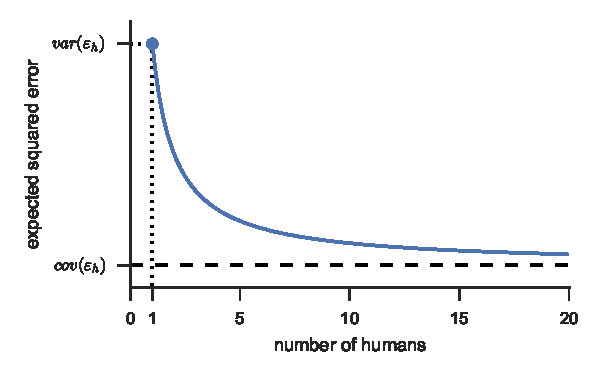
\includegraphics[width=0.7\textwidth]{proposal-humans_graph.pdf}
  \caption{
    Graph of the expected squared error of the average of forecasts by $n$ humans.
  }\label{fig: graph of humans only}
\end{figure}

First, let us examine the relationship between the expected squared errors of forecasts by a group of humans $H(n)$ and the number of humans $n$.
From (\ref{eq: expected squared error of humans}), the expected squared error takes $\varh$ when $n = 1$ and approaches $\covh$ when $n$ increases.
From the definition, $\varh \geq \covh$ holds, so (\ref{eq: expected squared error of humans}) decreases monotonically with $n \geq 1$.
Figure~\ref{fig: graph of humans only} shows the graph of $\MSE(H(n))$ when $n$ is a variable.

The expected squared error of a human-machine ensemble also approaches $\covh$ when $n \to \infty$ from (\ref{eq: expected squared error}).
And it takes $\varm$ when $n = 0$.
However, whether $\varm$ or $\covh$ is greater is different depending on $\x$, and sometimes (\ref{eq: expected squared error}) has a local minimum.

If (\ref{eq: expected squared error}) has a local minimum, the optimal number of humans $n^\ast$ always exists.
The condition to have a local minimum is
\begin{equation}
  \covmh < \frac{3\covh - \varh}{2}.
  \label{eq: condition}
\end{equation}
When taking the local minimum, $n$ is
\begin{equation}
  N^\ast(\x)
    = \frac
        {2var(\varepsilon_\theta|\x) - var(\varepsilon_h) + cov(\varepsilon_h) - 2cov(\varepsilon_\theta,\varepsilon_h)}
        {3 cov(\varepsilon_h) - var(\varepsilon_h) - 2 cov(\varepsilon_\theta,\varepsilon_h)}.
\end{equation}
If $N^\ast(\x)$ is greater than $0$, the optimal $n$ is $N^\ast(\x)$, and if $N^\ast(\x)$ is less than $0$, the optimal $n$ is $0$.
That is, $n^\ast$ that minimizes the expected squared error when (\ref{eq: expected squared error}) has a local minimum is
\begin{equation}
  n^\ast =
    \begin{cases}
      0 & (N^\ast(\x) <= 0) \\
      N^\ast(\x) & (N^\ast(\x) > 0).
    \end{cases}
\end{equation}

If (\ref{eq: condition}) does not hold, the optimal $n$ does not always exist.
In this case, the optimal $n$ is $0$ when $\varm \leq \covh$, and the optimal $n$ does not exist when $\varm > \covh$.
When $n^\ast$ does not exist, you can make the expected squared error close to $\covh$ by increasing $n$.

\begin{figure}
  \centering
  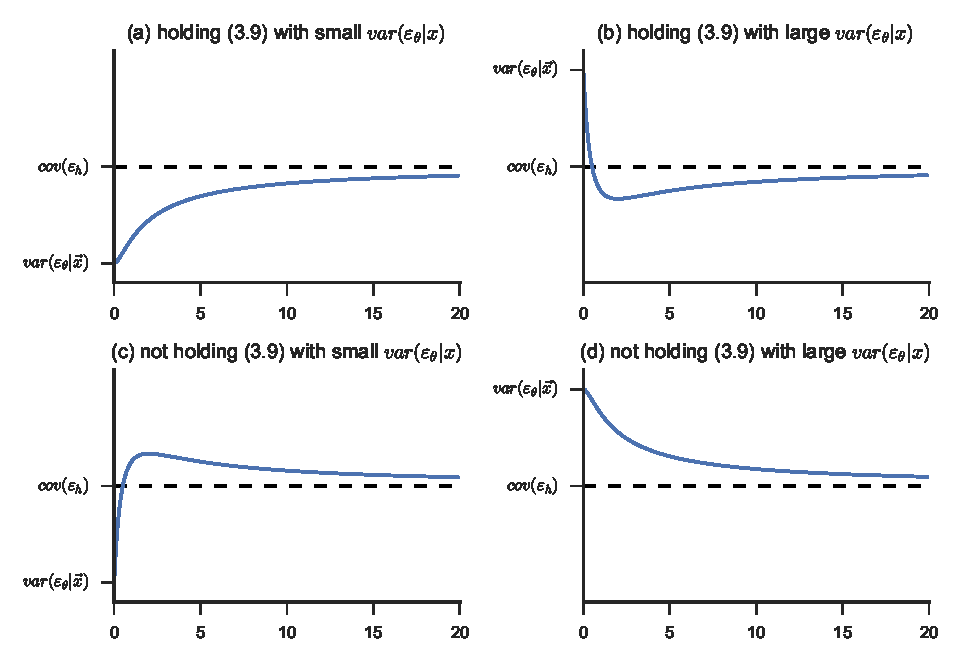
\includegraphics[width=\textwidth]{proposal-ensemble_graph.pdf}
  \caption{
    Approximate form of graphs about the expected squared errors of ensembles with $n$ as a variable.
    The upper two are cases where the condition (\ref{eq: condition}) holds, and $n^\ast = 0$ in (a) and $n^\ast = N^\ast(\x)$ in (b).
    The lower two are cases where the condition (\ref{eq: condition}) does not hold, and $n^\ast = 0$ in (c) and $n^\ast$ does not exist in (d).
  }\label{fig: graph of ensemble}
\end{figure}

Figure~\ref{fig: graph of ensemble} shows four graphs that have different optimal $n$.
These are grasped by adding a machine forecast to Figure~\ref{fig: graph of humans only} as the case of $n=0$.
The parameters related to machine forecasts $\varm$ and $\covmh$ influence the values near $n = 0$.
In particular, due to (\ref{eq: condition}), if $\covmh$ is sufficient smaller than the parameters related only to humans, that is, if the forecasts between a machine and humans are sufficiently different, (\ref{eq: expected squared error}) has local minimum.
\end{document}
